\section{Präzession}

Im folgenden wird das Produkt \(\omega_3 \cdot \omega_p\) gegen \(\omega_3\) aufgetragen, wobei \(\omega_p = \\
\begin{figure}[h]
    \centering
    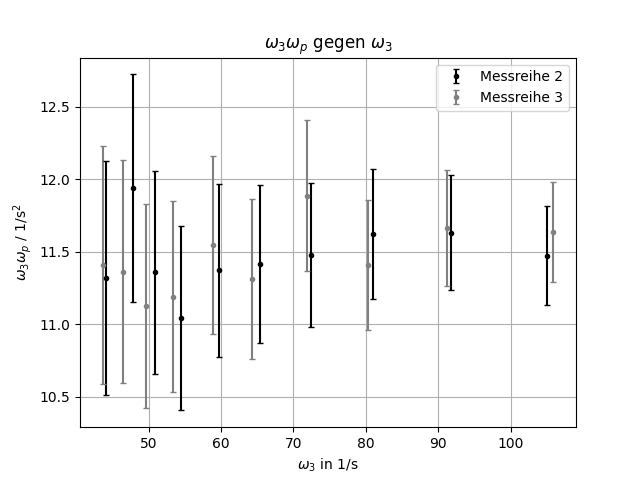
\includegraphics[scale=0.5]{6.3/Figure_1.png}
    \caption{Das berechnete Produkt \(\omega_3 \cdot \omega_p\) gegen \(\omega_3\) aufgetragen}
\end{figure}
\\
Es fällt auf, dass die Werte sehr nahe beieinander liegen. Dies läst vermuten, dass es sich bei dem Berechneten Produkt um eine Konstane handelt.
Die Fehler in der Zeichnung zeigen außerdem nur die Reinen Fehler der Messgeräte an, nicht jedoch die Fehler der der Messperson beim messen der einzelnen Gößen unterlaufen sind.

Um nun genauen Fehler der Größe \(\omega_3 \cdot \omega_p\) zu ermitteln bedienen wir uns der Statistik.\\
\begin{figure}[h]
    \centering
    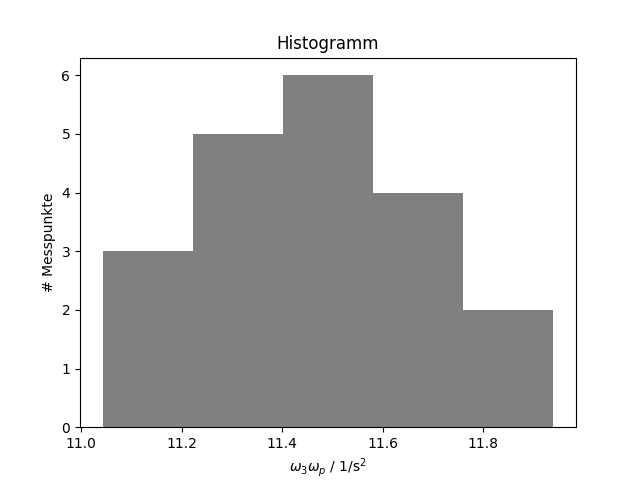
\includegraphics[scale=0.5]{6.3/Figure_2.png}
    \caption{Histogramm aller Messpunkte aus Messreihe eins und zwei.}
\end{figure}
\\
Für den Mittelwert ergibt sich: \(\overline{\omega_3 \cdot \omega_p} = 0,29028 \) und für die Standatabweichung glit: \( s = 0,0012889\).

Somit ergibt sich der Wert: \( \omega_3 \cdot \omega_p = (0,290 \pm 0,001) Hz^2\).